% Options for packages loaded elsewhere
\PassOptionsToPackage{unicode}{hyperref}
\PassOptionsToPackage{hyphens}{url}
%
\documentclass[
]{article}
\usepackage{amsmath,amssymb}
\usepackage{lmodern}
\usepackage{iftex}
\ifPDFTeX
  \usepackage[T1]{fontenc}
  \usepackage[utf8]{inputenc}
  \usepackage{textcomp} % provide euro and other symbols
\else % if luatex or xetex
  \usepackage{unicode-math}
  \defaultfontfeatures{Scale=MatchLowercase}
  \defaultfontfeatures[\rmfamily]{Ligatures=TeX,Scale=1}
\fi
% Use upquote if available, for straight quotes in verbatim environments
\IfFileExists{upquote.sty}{\usepackage{upquote}}{}
\IfFileExists{microtype.sty}{% use microtype if available
  \usepackage[]{microtype}
  \UseMicrotypeSet[protrusion]{basicmath} % disable protrusion for tt fonts
}{}
\makeatletter
\@ifundefined{KOMAClassName}{% if non-KOMA class
  \IfFileExists{parskip.sty}{%
    \usepackage{parskip}
  }{% else
    \setlength{\parindent}{0pt}
    \setlength{\parskip}{6pt plus 2pt minus 1pt}}
}{% if KOMA class
  \KOMAoptions{parskip=half}}
\makeatother
\usepackage{xcolor}
\IfFileExists{xurl.sty}{\usepackage{xurl}}{} % add URL line breaks if available
\IfFileExists{bookmark.sty}{\usepackage{bookmark}}{\usepackage{hyperref}}
\hypersetup{
  pdftitle={Assignment 6},
  pdfauthor={Guillermo Mercon},
  hidelinks,
  pdfcreator={LaTeX via pandoc}}
\urlstyle{same} % disable monospaced font for URLs
\usepackage[margin=1in]{geometry}
\usepackage{color}
\usepackage{fancyvrb}
\newcommand{\VerbBar}{|}
\newcommand{\VERB}{\Verb[commandchars=\\\{\}]}
\DefineVerbatimEnvironment{Highlighting}{Verbatim}{commandchars=\\\{\}}
% Add ',fontsize=\small' for more characters per line
\usepackage{framed}
\definecolor{shadecolor}{RGB}{248,248,248}
\newenvironment{Shaded}{\begin{snugshade}}{\end{snugshade}}
\newcommand{\AlertTok}[1]{\textcolor[rgb]{0.94,0.16,0.16}{#1}}
\newcommand{\AnnotationTok}[1]{\textcolor[rgb]{0.56,0.35,0.01}{\textbf{\textit{#1}}}}
\newcommand{\AttributeTok}[1]{\textcolor[rgb]{0.77,0.63,0.00}{#1}}
\newcommand{\BaseNTok}[1]{\textcolor[rgb]{0.00,0.00,0.81}{#1}}
\newcommand{\BuiltInTok}[1]{#1}
\newcommand{\CharTok}[1]{\textcolor[rgb]{0.31,0.60,0.02}{#1}}
\newcommand{\CommentTok}[1]{\textcolor[rgb]{0.56,0.35,0.01}{\textit{#1}}}
\newcommand{\CommentVarTok}[1]{\textcolor[rgb]{0.56,0.35,0.01}{\textbf{\textit{#1}}}}
\newcommand{\ConstantTok}[1]{\textcolor[rgb]{0.00,0.00,0.00}{#1}}
\newcommand{\ControlFlowTok}[1]{\textcolor[rgb]{0.13,0.29,0.53}{\textbf{#1}}}
\newcommand{\DataTypeTok}[1]{\textcolor[rgb]{0.13,0.29,0.53}{#1}}
\newcommand{\DecValTok}[1]{\textcolor[rgb]{0.00,0.00,0.81}{#1}}
\newcommand{\DocumentationTok}[1]{\textcolor[rgb]{0.56,0.35,0.01}{\textbf{\textit{#1}}}}
\newcommand{\ErrorTok}[1]{\textcolor[rgb]{0.64,0.00,0.00}{\textbf{#1}}}
\newcommand{\ExtensionTok}[1]{#1}
\newcommand{\FloatTok}[1]{\textcolor[rgb]{0.00,0.00,0.81}{#1}}
\newcommand{\FunctionTok}[1]{\textcolor[rgb]{0.00,0.00,0.00}{#1}}
\newcommand{\ImportTok}[1]{#1}
\newcommand{\InformationTok}[1]{\textcolor[rgb]{0.56,0.35,0.01}{\textbf{\textit{#1}}}}
\newcommand{\KeywordTok}[1]{\textcolor[rgb]{0.13,0.29,0.53}{\textbf{#1}}}
\newcommand{\NormalTok}[1]{#1}
\newcommand{\OperatorTok}[1]{\textcolor[rgb]{0.81,0.36,0.00}{\textbf{#1}}}
\newcommand{\OtherTok}[1]{\textcolor[rgb]{0.56,0.35,0.01}{#1}}
\newcommand{\PreprocessorTok}[1]{\textcolor[rgb]{0.56,0.35,0.01}{\textit{#1}}}
\newcommand{\RegionMarkerTok}[1]{#1}
\newcommand{\SpecialCharTok}[1]{\textcolor[rgb]{0.00,0.00,0.00}{#1}}
\newcommand{\SpecialStringTok}[1]{\textcolor[rgb]{0.31,0.60,0.02}{#1}}
\newcommand{\StringTok}[1]{\textcolor[rgb]{0.31,0.60,0.02}{#1}}
\newcommand{\VariableTok}[1]{\textcolor[rgb]{0.00,0.00,0.00}{#1}}
\newcommand{\VerbatimStringTok}[1]{\textcolor[rgb]{0.31,0.60,0.02}{#1}}
\newcommand{\WarningTok}[1]{\textcolor[rgb]{0.56,0.35,0.01}{\textbf{\textit{#1}}}}
\usepackage{graphicx}
\makeatletter
\def\maxwidth{\ifdim\Gin@nat@width>\linewidth\linewidth\else\Gin@nat@width\fi}
\def\maxheight{\ifdim\Gin@nat@height>\textheight\textheight\else\Gin@nat@height\fi}
\makeatother
% Scale images if necessary, so that they will not overflow the page
% margins by default, and it is still possible to overwrite the defaults
% using explicit options in \includegraphics[width, height, ...]{}
\setkeys{Gin}{width=\maxwidth,height=\maxheight,keepaspectratio}
% Set default figure placement to htbp
\makeatletter
\def\fps@figure{htbp}
\makeatother
\setlength{\emergencystretch}{3em} % prevent overfull lines
\providecommand{\tightlist}{%
  \setlength{\itemsep}{0pt}\setlength{\parskip}{0pt}}
\setcounter{secnumdepth}{-\maxdimen} % remove section numbering
\ifLuaTeX
  \usepackage{selnolig}  % disable illegal ligatures
\fi

\title{Assignment 6}
\author{Guillermo Mercon}
\date{2022-07-24}

\begin{document}
\maketitle

{
\setcounter{tocdepth}{2}
\tableofcontents
}
\begin{Shaded}
\begin{Highlighting}[]
\CommentTok{\# Add any packages you want in this chunk:}

\FunctionTok{library}\NormalTok{(readr)}
\FunctionTok{library}\NormalTok{(gvlma)}
\FunctionTok{library}\NormalTok{(MASS)}
\FunctionTok{library}\NormalTok{(leaps)}
\FunctionTok{library}\NormalTok{(car)}
\end{Highlighting}
\end{Shaded}

\begin{verbatim}
## Loading required package: carData
\end{verbatim}

We are going to look at the property prices for Orange County. From
there we are going to try and predict the sales price by linear
regression.

\hypertarget{importing-data}{%
\section{Importing Data}\label{importing-data}}

Bring in the data and make sure the data types are correct. If not, make
the proper changes. The file is located within this project.
\emph{data/prop\_prices\_reduced.csv}

\begin{Shaded}
\begin{Highlighting}[]
\NormalTok{prop\_prices\_reduced }\OtherTok{\textless{}{-}} \FunctionTok{read\_csv}\NormalTok{(}\StringTok{"\textasciitilde{}/GitHub/ECO5445SU22/Assignment06/data/prop\_prices\_reduced.csv"}\NormalTok{)}
\end{Highlighting}
\end{Shaded}

\begin{verbatim}
## Rows: 1000 Columns: 8
## -- Column specification --------------------------------------------------------
## Delimiter: ","
## dbl (8): sale_def, bed, bath, area_heated, area, dist_cbd, dist_lakes, pool
## 
## i Use `spec()` to retrieve the full column specification for this data.
## i Specify the column types or set `show_col_types = FALSE` to quiet this message.
\end{verbatim}

\begin{Shaded}
\begin{Highlighting}[]
\FunctionTok{View}\NormalTok{(prop\_prices\_reduced)}

\NormalTok{prop\_prices\_reduced}\SpecialCharTok{$}\NormalTok{sale\_def }\OtherTok{\textless{}{-}}\NormalTok{ prop\_prices\_reduced}\SpecialCharTok{$}\NormalTok{sale\_def}\SpecialCharTok{/}\DecValTok{1000}

\FunctionTok{attach}\NormalTok{(prop\_prices\_reduced)}
\end{Highlighting}
\end{Shaded}

\begin{itemize}
\tightlist
\item
  Here I changed sale\_def and scaled those prices down by 1000. This
  will help the scale of the graphs later so the x and y borders are not
  so large.
\end{itemize}

\hypertarget{plotting}{%
\section{Plotting}\label{plotting}}

Plot histograms for all variables. Additionally, add scatter plots for
the relationships between all quantitative variables.

\begin{itemize}
\tightlist
\item
  Here I included all the histograms and a scatterplot which has all
  relationships between each variable on one page. I also included some
  of the more important scatterplots, mainly the deflated sales by each
  variable.
\end{itemize}

\begin{Shaded}
\begin{Highlighting}[]
\FunctionTok{hist}\NormalTok{(sale\_def, }\AttributeTok{breaks =} \StringTok{"fd"}\NormalTok{,}\AttributeTok{main =} \StringTok{"Histogram of Sales Deflated"}\NormalTok{)}
\end{Highlighting}
\end{Shaded}

\includegraphics{Assignment06_files/figure-latex/unnamed-chunk-2-1.pdf}

\begin{Shaded}
\begin{Highlighting}[]
\FunctionTok{hist}\NormalTok{(bed, }\AttributeTok{main =} \StringTok{"Histogram of \# of Beds"}\NormalTok{)}
\end{Highlighting}
\end{Shaded}

\includegraphics{Assignment06_files/figure-latex/unnamed-chunk-2-2.pdf}

\begin{Shaded}
\begin{Highlighting}[]
\FunctionTok{hist}\NormalTok{(bath, }\AttributeTok{main =} \StringTok{"Histogram of Baths"}\NormalTok{)}
\end{Highlighting}
\end{Shaded}

\includegraphics{Assignment06_files/figure-latex/unnamed-chunk-2-3.pdf}

\begin{Shaded}
\begin{Highlighting}[]
\FunctionTok{hist}\NormalTok{(area\_heated, }\AttributeTok{main =} \StringTok{"Histogram of Area Heated"}\NormalTok{)}
\end{Highlighting}
\end{Shaded}

\includegraphics{Assignment06_files/figure-latex/unnamed-chunk-2-4.pdf}

\begin{Shaded}
\begin{Highlighting}[]
\FunctionTok{hist}\NormalTok{(area, }\AttributeTok{main =} \StringTok{"Histogram of Area"}\NormalTok{)}
\end{Highlighting}
\end{Shaded}

\includegraphics{Assignment06_files/figure-latex/unnamed-chunk-2-5.pdf}

\begin{Shaded}
\begin{Highlighting}[]
\FunctionTok{hist}\NormalTok{(dist\_cbd, }\AttributeTok{main =} \StringTok{"Histogram of Distance to CBD"}\NormalTok{)}
\end{Highlighting}
\end{Shaded}

\includegraphics{Assignment06_files/figure-latex/unnamed-chunk-2-6.pdf}

\begin{Shaded}
\begin{Highlighting}[]
\FunctionTok{hist}\NormalTok{(dist\_lakes, }\AttributeTok{main =} \StringTok{"Histogram of Distance to Lakes"}\NormalTok{)}
\end{Highlighting}
\end{Shaded}

\includegraphics{Assignment06_files/figure-latex/unnamed-chunk-2-7.pdf}

\begin{Shaded}
\begin{Highlighting}[]
\FunctionTok{hist}\NormalTok{(pool, }\AttributeTok{main =} \StringTok{"Histogram of Houses with Pools"}\NormalTok{)}
\end{Highlighting}
\end{Shaded}

\includegraphics{Assignment06_files/figure-latex/unnamed-chunk-2-8.pdf}

\begin{Shaded}
\begin{Highlighting}[]
\FunctionTok{plot}\NormalTok{(prop\_prices\_reduced, }\AttributeTok{main =} \StringTok{"Scatterplot of All Relationships"}\NormalTok{)}
\end{Highlighting}
\end{Shaded}

\includegraphics{Assignment06_files/figure-latex/unnamed-chunk-2-9.pdf}

\begin{Shaded}
\begin{Highlighting}[]
\FunctionTok{plot}\NormalTok{(bed,sale\_def, }\AttributeTok{main =} \StringTok{"Sale Price by \# of Beds"}\NormalTok{)}
\end{Highlighting}
\end{Shaded}

\includegraphics{Assignment06_files/figure-latex/unnamed-chunk-2-10.pdf}

\begin{Shaded}
\begin{Highlighting}[]
\FunctionTok{plot}\NormalTok{(bath,sale\_def, }\AttributeTok{main =} \StringTok{"Sale Price by \# of Bathrooms"}\NormalTok{)}
\end{Highlighting}
\end{Shaded}

\includegraphics{Assignment06_files/figure-latex/unnamed-chunk-2-11.pdf}

\begin{Shaded}
\begin{Highlighting}[]
\FunctionTok{plot}\NormalTok{(area,sale\_def, }\AttributeTok{main =} \StringTok{"Sale Price by Area"}\NormalTok{)}
\end{Highlighting}
\end{Shaded}

\includegraphics{Assignment06_files/figure-latex/unnamed-chunk-2-12.pdf}

\begin{Shaded}
\begin{Highlighting}[]
\FunctionTok{plot}\NormalTok{(area\_heated,sale\_def, }\AttributeTok{main =} \StringTok{"Sale Price by Area Heated"}\NormalTok{)}
\end{Highlighting}
\end{Shaded}

\includegraphics{Assignment06_files/figure-latex/unnamed-chunk-2-13.pdf}

\begin{Shaded}
\begin{Highlighting}[]
\FunctionTok{plot}\NormalTok{(dist\_cbd,sale\_def, }\AttributeTok{main =} \StringTok{"Sale Price by Distance to Central Business District"}\NormalTok{)}
\end{Highlighting}
\end{Shaded}

\includegraphics{Assignment06_files/figure-latex/unnamed-chunk-2-14.pdf}

\begin{Shaded}
\begin{Highlighting}[]
\FunctionTok{plot}\NormalTok{(dist\_lakes,sale\_def, }\AttributeTok{main =} \StringTok{"Sale Price by Distance to Lake"}\NormalTok{)}
\end{Highlighting}
\end{Shaded}

\includegraphics{Assignment06_files/figure-latex/unnamed-chunk-2-15.pdf}

\begin{Shaded}
\begin{Highlighting}[]
\FunctionTok{plot}\NormalTok{(pool,sale\_def, }\AttributeTok{main =} \StringTok{"Sale Price by Pool"}\NormalTok{)}
\end{Highlighting}
\end{Shaded}

\includegraphics{Assignment06_files/figure-latex/unnamed-chunk-2-16.pdf}

\begin{Shaded}
\begin{Highlighting}[]
\FunctionTok{plot}\NormalTok{(area,area\_heated, }\AttributeTok{main =} \StringTok{"Area Heated by Total Area"}\NormalTok{)}
\end{Highlighting}
\end{Shaded}

\includegraphics{Assignment06_files/figure-latex/unnamed-chunk-2-17.pdf}

\hypertarget{summary-statistics}{%
\section{Summary Statistics}\label{summary-statistics}}

Provide basic summary statistics for univariate analysis. Also, provide
the correlation between all the quantitative variables.

\begin{Shaded}
\begin{Highlighting}[]
\FunctionTok{summary}\NormalTok{(prop\_prices\_reduced)}
\end{Highlighting}
\end{Shaded}

\begin{verbatim}
##     sale_def           bed             bath        area_heated   
##  Min.   :  15.3   Min.   :1.000   Min.   :1.000   Min.   :  650  
##  1st Qu.: 115.6   1st Qu.:3.000   1st Qu.:2.000   1st Qu.: 1387  
##  Median : 151.1   Median :3.000   Median :2.000   Median : 1744  
##  Mean   : 200.3   Mean   :3.398   Mean   :2.248   Mean   : 1955  
##  3rd Qu.: 213.9   3rd Qu.:4.000   3rd Qu.:2.500   3rd Qu.: 2301  
##  Max.   :7630.0   Max.   :7.000   Max.   :8.000   Max.   :10796  
##       area           dist_cbd         dist_lakes           pool      
##  Min.   :  1307   Min.   :  598.2   Min.   :  16.74   Min.   :0.000  
##  1st Qu.:  6498   1st Qu.: 9701.7   1st Qu.: 314.86   1st Qu.:0.000  
##  Median :  8733   Median :14552.0   Median : 638.82   Median :0.000  
##  Mean   : 10565   Mean   :14382.9   Mean   :1403.54   Mean   :0.229  
##  3rd Qu.: 11250   3rd Qu.:19369.2   3rd Qu.:1735.35   3rd Qu.:0.000  
##  Max.   :269496   Max.   :36107.6   Max.   :8206.79   Max.   :1.000
\end{verbatim}

\begin{Shaded}
\begin{Highlighting}[]
\FunctionTok{cor}\NormalTok{(prop\_prices\_reduced)}
\end{Highlighting}
\end{Shaded}

\begin{verbatim}
##                sale_def        bed        bath area_heated        area
## sale_def     1.00000000 0.32557109  0.58731596  0.69201080  0.34354392
## bed          0.32557109 1.00000000  0.64449531  0.66911599  0.10437035
## bath         0.58731596 0.64449531  1.00000000  0.83255359  0.19298319
## area_heated  0.69201080 0.66911599  0.83255359  1.00000000  0.30184325
## area         0.34354392 0.10437035  0.19298319  0.30184325  1.00000000
## dist_cbd     0.05263700 0.23328277  0.24220637  0.25494517  0.08648327
## dist_lakes  -0.08857844 0.03747888 -0.02109154 -0.04092947 -0.15432291
## pool         0.27749823 0.31299930  0.38722523  0.43899880  0.19200110
##               dist_cbd  dist_lakes        pool
## sale_def    0.05263700 -0.08857844  0.27749823
## bed         0.23328277  0.03747888  0.31299930
## bath        0.24220637 -0.02109154  0.38722523
## area_heated 0.25494517 -0.04092947  0.43899880
## area        0.08648327 -0.15432291  0.19200110
## dist_cbd    1.00000000  0.26520451  0.11442899
## dist_lakes  0.26520451  1.00000000 -0.04295257
## pool        0.11442899 -0.04295257  1.00000000
\end{verbatim}

\hypertarget{regression-analysis}{%
\section{Regression Analysis}\label{regression-analysis}}

Run a regression with all the variables included. Print results of the
regression.

\begin{Shaded}
\begin{Highlighting}[]
\FunctionTok{scatterplotMatrix}\NormalTok{(prop\_prices\_reduced, }\AttributeTok{smooth =} \ConstantTok{FALSE}\NormalTok{, }\AttributeTok{main =} \StringTok{"Scatterplot Matrix"}\NormalTok{)}
\end{Highlighting}
\end{Shaded}

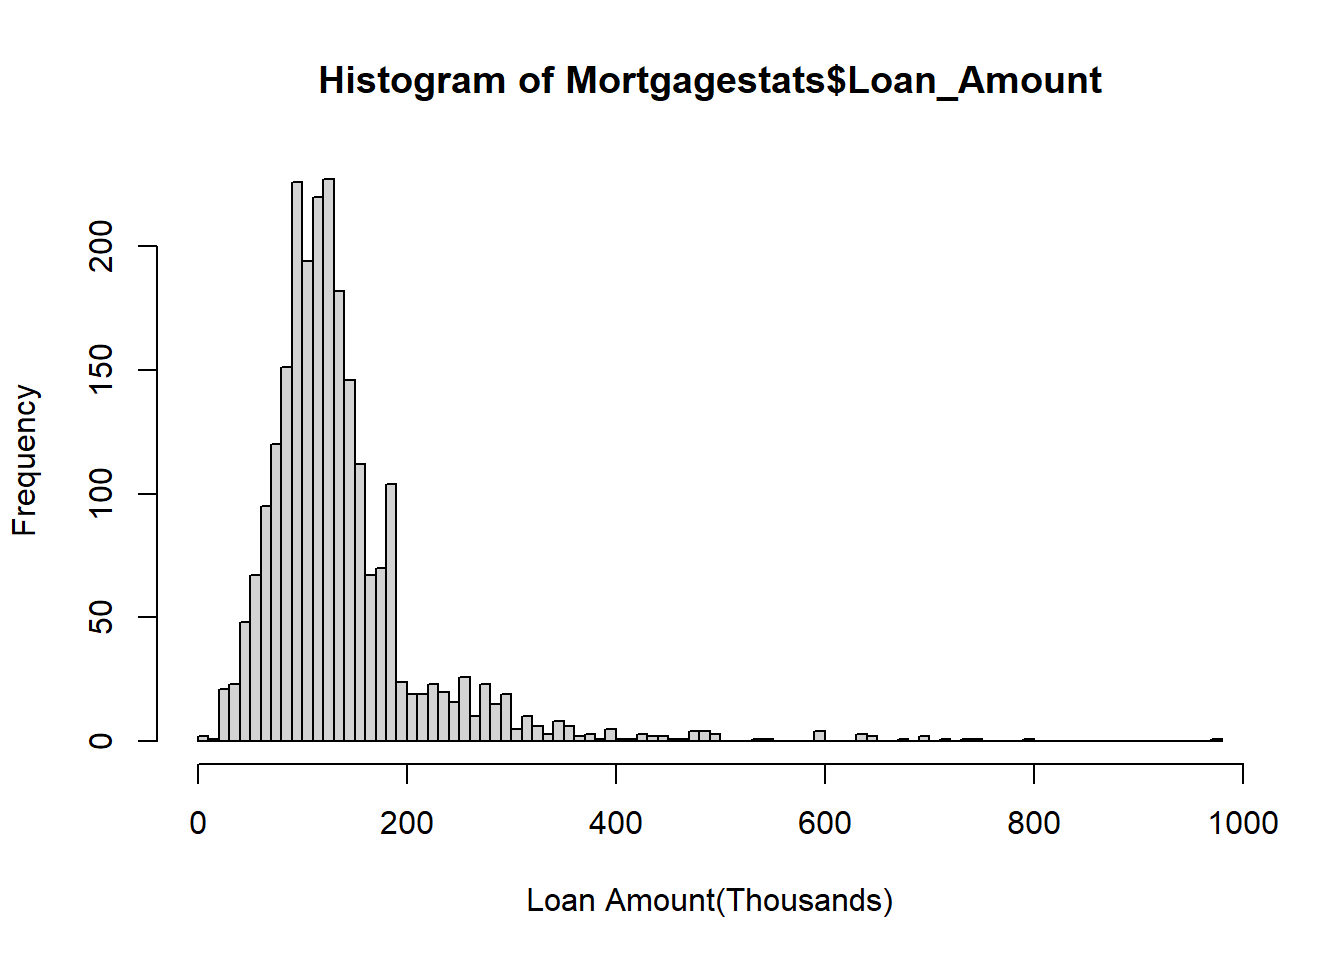
\includegraphics{Assignment06_files/figure-latex/unnamed-chunk-4-1.pdf}

\begin{Shaded}
\begin{Highlighting}[]
\NormalTok{fit }\OtherTok{\textless{}{-}}\FunctionTok{lm}\NormalTok{(sale\_def }\SpecialCharTok{\textasciitilde{}}\NormalTok{ bed }\SpecialCharTok{+}\NormalTok{ bath }\SpecialCharTok{+}\NormalTok{ area\_heated }\SpecialCharTok{+}\NormalTok{ area }\SpecialCharTok{+}\NormalTok{ dist\_cbd }\SpecialCharTok{+}\NormalTok{ dist\_lakes }\SpecialCharTok{+}\NormalTok{ pool,}\AttributeTok{data =}\NormalTok{ prop\_prices\_reduced)}

\FunctionTok{summary}\NormalTok{(fit)}
\end{Highlighting}
\end{Shaded}

\begin{verbatim}
## 
## Call:
## lm(formula = sale_def ~ bed + bath + area_heated + area + dist_cbd + 
##     dist_lakes + pool, data = prop_prices_reduced)
## 
## Residuals:
##    Min     1Q Median     3Q    Max 
## -765.2  -56.0    9.8   63.8 4954.8 
## 
## Coefficients:
##               Estimate Std. Error t value Pr(>|t|)    
## (Intercept) -5.890e+01  3.093e+01  -1.904 0.057170 .  
## bed         -8.492e+01  1.087e+01  -7.810 1.45e-14 ***
## bath         5.449e+01  1.507e+01   3.616 0.000315 ***
## area_heated  2.439e-01  1.430e-02  17.054  < 2e-16 ***
## area         3.548e-03  5.958e-04   5.955 3.61e-09 ***
## dist_cbd    -5.849e-03  1.090e-03  -5.366 1.00e-07 ***
## dist_lakes   9.651e-04  3.810e-03   0.253 0.800091    
## pool        -2.776e+01  1.640e+01  -1.693 0.090787 .  
## ---
## Signif. codes:  0 '***' 0.001 '**' 0.01 '*' 0.05 '.' 0.1 ' ' 1
## 
## Residual standard error: 194.9 on 992 degrees of freedom
## Multiple R-squared:  0.547,  Adjusted R-squared:  0.5438 
## F-statistic: 171.2 on 7 and 992 DF,  p-value: < 2.2e-16
\end{verbatim}

Which of the variables tested significant at the 95\% level? Looking at
the results and answering outside of the chunk is sufficient.

Answer: The variables that tested significant at the 95\% level include
bed, bath, area heated, area, distance to cbd, and pool. This leaves
distance to lakes as insignificant. Another thing to note is that pool
tested significant at 95\% while the rest of the variables tested
significant at up to 99.99\%

\hypertarget{evaluating-the-model}{%
\subsection{Evaluating the model}\label{evaluating-the-model}}

As is, are any of the Gauss-Markov assumptions violated? If so, which
ones? How can you fix the issues?

\begin{Shaded}
\begin{Highlighting}[]
\NormalTok{opar }\OtherTok{\textless{}{-}} \FunctionTok{par}\NormalTok{(}\AttributeTok{no.readonly =} \ConstantTok{TRUE}\NormalTok{)}

\FunctionTok{par}\NormalTok{(}\AttributeTok{mfrow =} \FunctionTok{c}\NormalTok{(}\DecValTok{2}\NormalTok{, }\DecValTok{2}\NormalTok{))}
\FunctionTok{plot}\NormalTok{(fit)}
\end{Highlighting}
\end{Shaded}

\includegraphics{Assignment06_files/figure-latex/unnamed-chunk-5-1.pdf}

\begin{Shaded}
\begin{Highlighting}[]
\FunctionTok{par}\NormalTok{(opar)}

\FunctionTok{durbinWatsonTest}\NormalTok{(fit)}
\end{Highlighting}
\end{Shaded}

\begin{verbatim}
##  lag Autocorrelation D-W Statistic p-value
##    1    -0.008920317      2.017485   0.728
##  Alternative hypothesis: rho != 0
\end{verbatim}

\begin{Shaded}
\begin{Highlighting}[]
\NormalTok{gvmodel }\OtherTok{\textless{}{-}} \FunctionTok{gvlma}\NormalTok{(fit)}
\FunctionTok{summary}\NormalTok{(gvmodel)}
\end{Highlighting}
\end{Shaded}

\begin{verbatim}
## 
## Call:
## lm(formula = sale_def ~ bed + bath + area_heated + area + dist_cbd + 
##     dist_lakes + pool, data = prop_prices_reduced)
## 
## Residuals:
##    Min     1Q Median     3Q    Max 
## -765.2  -56.0    9.8   63.8 4954.8 
## 
## Coefficients:
##               Estimate Std. Error t value Pr(>|t|)    
## (Intercept) -5.890e+01  3.093e+01  -1.904 0.057170 .  
## bed         -8.492e+01  1.087e+01  -7.810 1.45e-14 ***
## bath         5.449e+01  1.507e+01   3.616 0.000315 ***
## area_heated  2.439e-01  1.430e-02  17.054  < 2e-16 ***
## area         3.548e-03  5.958e-04   5.955 3.61e-09 ***
## dist_cbd    -5.849e-03  1.090e-03  -5.366 1.00e-07 ***
## dist_lakes   9.651e-04  3.810e-03   0.253 0.800091    
## pool        -2.776e+01  1.640e+01  -1.693 0.090787 .  
## ---
## Signif. codes:  0 '***' 0.001 '**' 0.01 '*' 0.05 '.' 0.1 ' ' 1
## 
## Residual standard error: 194.9 on 992 degrees of freedom
## Multiple R-squared:  0.547,  Adjusted R-squared:  0.5438 
## F-statistic: 171.2 on 7 and 992 DF,  p-value: < 2.2e-16
## 
## 
## ASSESSMENT OF THE LINEAR MODEL ASSUMPTIONS
## USING THE GLOBAL TEST ON 4 DEGREES-OF-FREEDOM:
## Level of Significance =  0.05 
## 
## Call:
##  gvlma(x = fit) 
## 
##                        Value p-value                   Decision
## Global Stat        7497980.4       0 Assumptions NOT satisfied!
## Skewness             45659.6       0 Assumptions NOT satisfied!
## Kurtosis           7450926.5       0 Assumptions NOT satisfied!
## Link Function          782.2       0 Assumptions NOT satisfied!
## Heteroscedasticity     612.1       0 Assumptions NOT satisfied!
\end{verbatim}

\begin{Shaded}
\begin{Highlighting}[]
\FunctionTok{qqPlot}\NormalTok{(fit, }\AttributeTok{labels =} \ConstantTok{FALSE}\NormalTok{, }\AttributeTok{simulate =} \ConstantTok{TRUE}\NormalTok{, }\AttributeTok{main =} \StringTok{"Q{-}Q Plot"}\NormalTok{)}
\end{Highlighting}
\end{Shaded}

\includegraphics{Assignment06_files/figure-latex/unnamed-chunk-5-2.pdf}

\begin{verbatim}
## [1]  7 37
\end{verbatim}

\begin{itemize}
\item
  It appears as though we have an outlier at index number 37. This
  appears to be causing a violation of Gauss Markov assumption \#1. If
  we remove this outlier we will be studying a more homogenous sample.
\item
  We also see that distance to lakes is not significant. This is a
  violation of Gauss Markov assumption \#3. I will adjust this by trying
  several variations. First we will change ``distance to lakes'' to a
  percentage by dividing the distance by the mean distance to lakes. I
  will then try to change the formula so that distance to lakes is
  included as a quadratic variable. Finally I will take the original
  formula and take the log of the deflated sales and the log of the
  distance to lakes. I will then compare the two formulas to see which
  has a higher R\^{}2 and more significance.
\end{itemize}

\hypertarget{new-model}{%
\subsection{New Model}\label{new-model}}

Based off of your findings in the previous section, make changes to the
variables, the functional form, etc.

\begin{Shaded}
\begin{Highlighting}[]
\NormalTok{newdata }\OtherTok{\textless{}{-}}\NormalTok{ prop\_prices\_reduced[}\SpecialCharTok{{-}}\FunctionTok{c}\NormalTok{(}\DecValTok{37}\NormalTok{),]}
\NormalTok{newdata}\SpecialCharTok{$}\NormalTok{dist\_lakes }\OtherTok{\textless{}{-}}\NormalTok{ newdata}\SpecialCharTok{$}\NormalTok{dist\_lakes}\SpecialCharTok{/}\FunctionTok{mean}\NormalTok{(newdata}\SpecialCharTok{$}\NormalTok{dist\_lakes)}


\NormalTok{newfit1 }\OtherTok{\textless{}{-}}  \FunctionTok{lm}\NormalTok{(sale\_def }\SpecialCharTok{\textasciitilde{}}\NormalTok{ bed }\SpecialCharTok{+}\NormalTok{ bath }\SpecialCharTok{+}\NormalTok{ area\_heated }\SpecialCharTok{+}\NormalTok{ area }\SpecialCharTok{+}\NormalTok{ dist\_cbd }\SpecialCharTok{+}\NormalTok{ dist\_lakes }\SpecialCharTok{+}\NormalTok{ pool }\SpecialCharTok{+} \FunctionTok{I}\NormalTok{(dist\_lakes}\SpecialCharTok{\^{}}\DecValTok{2}\NormalTok{),}\AttributeTok{data =}\NormalTok{ newdata)}
\FunctionTok{summary}\NormalTok{(newfit1)}
\end{Highlighting}
\end{Shaded}

\begin{verbatim}
## 
## Call:
## lm(formula = sale_def ~ bed + bath + area_heated + area + dist_cbd + 
##     dist_lakes + pool + I(dist_lakes^2), data = newdata)
## 
## Residuals:
##     Min      1Q  Median      3Q     Max 
## -281.58  -41.72    0.54   35.34 1213.95 
## 
## Coefficients:
##                   Estimate Std. Error t value Pr(>|t|)    
## (Intercept)     -1.756e+01  1.538e+01  -1.142   0.2537    
## bed             -4.526e+01  5.295e+00  -8.548  < 2e-16 ***
## bath             5.651e+01  7.287e+00   7.755 2.19e-14 ***
## area_heated      1.436e-01  7.182e-03  19.996  < 2e-16 ***
## area             1.463e-03  2.907e-04   5.034 5.71e-07 ***
## dist_cbd        -3.759e-03  5.298e-04  -7.095 2.46e-12 ***
## dist_lakes      -1.351e+01  7.874e+00  -1.716   0.0864 .  
## pool             1.916e+01  7.959e+00   2.407   0.0163 *  
## I(dist_lakes^2)  2.298e+00  1.730e+00   1.329   0.1842    
## ---
## Signif. codes:  0 '***' 0.001 '**' 0.01 '*' 0.05 '.' 0.1 ' ' 1
## 
## Residual standard error: 94.08 on 990 degrees of freedom
## Multiple R-squared:  0.6862, Adjusted R-squared:  0.6837 
## F-statistic: 270.6 on 8 and 990 DF,  p-value: < 2.2e-16
\end{verbatim}

\begin{Shaded}
\begin{Highlighting}[]
\NormalTok{newfit2 }\OtherTok{\textless{}{-}}  \FunctionTok{lm}\NormalTok{(}\FunctionTok{log}\NormalTok{(sale\_def) }\SpecialCharTok{\textasciitilde{}}\NormalTok{ bed }\SpecialCharTok{+}\NormalTok{ bath }\SpecialCharTok{+}\NormalTok{ area\_heated }\SpecialCharTok{+}\NormalTok{ area }\SpecialCharTok{+}\NormalTok{ dist\_cbd }\SpecialCharTok{+} \FunctionTok{log}\NormalTok{(dist\_lakes) }\SpecialCharTok{+}\NormalTok{ pool, }\AttributeTok{data =}\NormalTok{ newdata)}
\FunctionTok{summary}\NormalTok{(newfit2)}
\end{Highlighting}
\end{Shaded}

\begin{verbatim}
## 
## Call:
## lm(formula = log(sale_def) ~ bed + bath + area_heated + area + 
##     dist_cbd + log(dist_lakes) + pool, data = newdata)
## 
## Residuals:
##      Min       1Q   Median       3Q      Max 
## -1.72664 -0.15869  0.00606  0.17284  1.03229 
## 
## Coefficients:
##                   Estimate Std. Error t value Pr(>|t|)    
## (Intercept)      4.082e+00  4.514e-02  90.421  < 2e-16 ***
## bed             -4.199e-02  1.574e-02  -2.668 0.007756 ** 
## bath             1.255e-01  2.161e-02   5.809 8.48e-09 ***
## area_heated      4.506e-04  2.126e-05  21.189  < 2e-16 ***
## area             2.480e-06  8.696e-07   2.852 0.004438 ** 
## dist_cbd        -5.869e-06  1.587e-06  -3.699 0.000228 ***
## log(dist_lakes) -2.328e-02  7.874e-03  -2.957 0.003180 ** 
## pool             1.326e-01  2.363e-02   5.612 2.60e-08 ***
## ---
## Signif. codes:  0 '***' 0.001 '**' 0.01 '*' 0.05 '.' 0.1 ' ' 1
## 
## Residual standard error: 0.2795 on 991 degrees of freedom
## Multiple R-squared:  0.7337, Adjusted R-squared:  0.7318 
## F-statistic:   390 on 7 and 991 DF,  p-value: < 2.2e-16
\end{verbatim}

\begin{Shaded}
\begin{Highlighting}[]
\FunctionTok{par}\NormalTok{(}\AttributeTok{mfrow =} \FunctionTok{c}\NormalTok{(}\DecValTok{2}\NormalTok{, }\DecValTok{2}\NormalTok{))}
\FunctionTok{plot}\NormalTok{(newfit1)}
\end{Highlighting}
\end{Shaded}

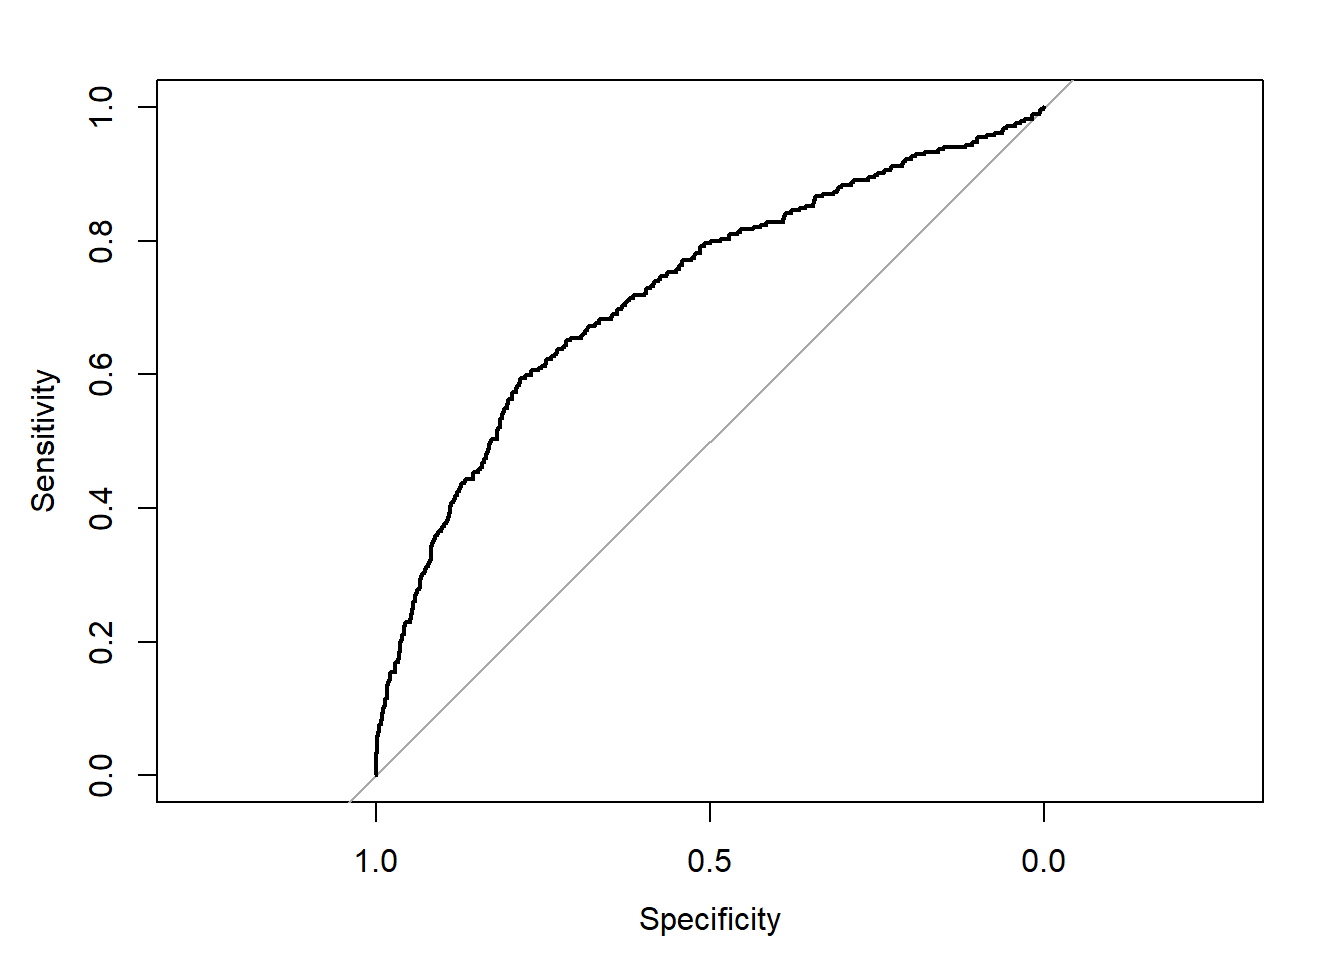
\includegraphics{Assignment06_files/figure-latex/unnamed-chunk-6-1.pdf}

\begin{Shaded}
\begin{Highlighting}[]
\FunctionTok{par}\NormalTok{(}\AttributeTok{mfrow =} \FunctionTok{c}\NormalTok{(}\DecValTok{2}\NormalTok{, }\DecValTok{2}\NormalTok{))}
\FunctionTok{plot}\NormalTok{(newfit2)}
\end{Highlighting}
\end{Shaded}

\includegraphics{Assignment06_files/figure-latex/unnamed-chunk-6-2.pdf}

\begin{Shaded}
\begin{Highlighting}[]
\FunctionTok{par}\NormalTok{(opar)}

\NormalTok{gvmodelnew1 }\OtherTok{\textless{}{-}} \FunctionTok{gvlma}\NormalTok{(newfit1)}
\FunctionTok{summary}\NormalTok{(gvmodelnew1)}
\end{Highlighting}
\end{Shaded}

\begin{verbatim}
## 
## Call:
## lm(formula = sale_def ~ bed + bath + area_heated + area + dist_cbd + 
##     dist_lakes + pool + I(dist_lakes^2), data = newdata)
## 
## Residuals:
##     Min      1Q  Median      3Q     Max 
## -281.58  -41.72    0.54   35.34 1213.95 
## 
## Coefficients:
##                   Estimate Std. Error t value Pr(>|t|)    
## (Intercept)     -1.756e+01  1.538e+01  -1.142   0.2537    
## bed             -4.526e+01  5.295e+00  -8.548  < 2e-16 ***
## bath             5.651e+01  7.287e+00   7.755 2.19e-14 ***
## area_heated      1.436e-01  7.182e-03  19.996  < 2e-16 ***
## area             1.463e-03  2.907e-04   5.034 5.71e-07 ***
## dist_cbd        -3.759e-03  5.298e-04  -7.095 2.46e-12 ***
## dist_lakes      -1.351e+01  7.874e+00  -1.716   0.0864 .  
## pool             1.916e+01  7.959e+00   2.407   0.0163 *  
## I(dist_lakes^2)  2.298e+00  1.730e+00   1.329   0.1842    
## ---
## Signif. codes:  0 '***' 0.001 '**' 0.01 '*' 0.05 '.' 0.1 ' ' 1
## 
## Residual standard error: 94.08 on 990 degrees of freedom
## Multiple R-squared:  0.6862, Adjusted R-squared:  0.6837 
## F-statistic: 270.6 on 8 and 990 DF,  p-value: < 2.2e-16
## 
## 
## ASSESSMENT OF THE LINEAR MODEL ASSUMPTIONS
## USING THE GLOBAL TEST ON 4 DEGREES-OF-FREEDOM:
## Level of Significance =  0.05 
## 
## Call:
##  gvlma(x = newfit1) 
## 
##                        Value p-value                   Decision
## Global Stat        1.217e+05  0.0000 Assumptions NOT satisfied!
## Skewness           3.752e+03  0.0000 Assumptions NOT satisfied!
## Kurtosis           1.176e+05  0.0000 Assumptions NOT satisfied!
## Link Function      3.548e+02  0.0000 Assumptions NOT satisfied!
## Heteroscedasticity 5.065e-01  0.4767    Assumptions acceptable.
\end{verbatim}

\begin{Shaded}
\begin{Highlighting}[]
\NormalTok{gvmodelnew2 }\OtherTok{\textless{}{-}} \FunctionTok{gvlma}\NormalTok{(newfit2)}
\FunctionTok{summary}\NormalTok{(gvmodelnew2)}
\end{Highlighting}
\end{Shaded}

\begin{verbatim}
## 
## Call:
## lm(formula = log(sale_def) ~ bed + bath + area_heated + area + 
##     dist_cbd + log(dist_lakes) + pool, data = newdata)
## 
## Residuals:
##      Min       1Q   Median       3Q      Max 
## -1.72664 -0.15869  0.00606  0.17284  1.03229 
## 
## Coefficients:
##                   Estimate Std. Error t value Pr(>|t|)    
## (Intercept)      4.082e+00  4.514e-02  90.421  < 2e-16 ***
## bed             -4.199e-02  1.574e-02  -2.668 0.007756 ** 
## bath             1.255e-01  2.161e-02   5.809 8.48e-09 ***
## area_heated      4.506e-04  2.126e-05  21.189  < 2e-16 ***
## area             2.480e-06  8.696e-07   2.852 0.004438 ** 
## dist_cbd        -5.869e-06  1.587e-06  -3.699 0.000228 ***
## log(dist_lakes) -2.328e-02  7.874e-03  -2.957 0.003180 ** 
## pool             1.326e-01  2.363e-02   5.612 2.60e-08 ***
## ---
## Signif. codes:  0 '***' 0.001 '**' 0.01 '*' 0.05 '.' 0.1 ' ' 1
## 
## Residual standard error: 0.2795 on 991 degrees of freedom
## Multiple R-squared:  0.7337, Adjusted R-squared:  0.7318 
## F-statistic:   390 on 7 and 991 DF,  p-value: < 2.2e-16
## 
## 
## ASSESSMENT OF THE LINEAR MODEL ASSUMPTIONS
## USING THE GLOBAL TEST ON 4 DEGREES-OF-FREEDOM:
## Level of Significance =  0.05 
## 
## Call:
##  gvlma(x = newfit2) 
## 
##                      Value   p-value                   Decision
## Global Stat        311.035 0.000e+00 Assumptions NOT satisfied!
## Skewness            19.671 9.197e-06 Assumptions NOT satisfied!
## Kurtosis           251.463 0.000e+00 Assumptions NOT satisfied!
## Link Function       37.778 7.925e-10 Assumptions NOT satisfied!
## Heteroscedasticity   2.122 1.452e-01    Assumptions acceptable.
\end{verbatim}

\begin{Shaded}
\begin{Highlighting}[]
\FunctionTok{qqPlot}\NormalTok{(newfit1, }\AttributeTok{labels =} \ConstantTok{FALSE}\NormalTok{, }\AttributeTok{simulate =} \ConstantTok{TRUE}\NormalTok{, }\AttributeTok{main =} \StringTok{"Q{-}Q Plot, Quadratic"}\NormalTok{)}
\end{Highlighting}
\end{Shaded}

\includegraphics{Assignment06_files/figure-latex/unnamed-chunk-6-3.pdf}

\begin{verbatim}
## [1] 213 637
\end{verbatim}

\begin{Shaded}
\begin{Highlighting}[]
\FunctionTok{qqPlot}\NormalTok{(newfit2, }\AttributeTok{labels =} \ConstantTok{FALSE}\NormalTok{, }\AttributeTok{simulate =} \ConstantTok{TRUE}\NormalTok{, }\AttributeTok{main =} \StringTok{"Q{-}Q Plot, Log"}\NormalTok{)}
\end{Highlighting}
\end{Shaded}

\includegraphics{Assignment06_files/figure-latex/unnamed-chunk-6-4.pdf}

\begin{verbatim}
## [1] 151 328
\end{verbatim}

\begin{itemize}
\tightlist
\item
  It appears as though the quadratic transformation brought the adjusted
  R squared up to .68 while the log transformation brought it up to .73.
  The log transformation also brings up the significance of distance to
  lakes to above 95\%. It also brings the residuals vs fitted values
  down to a much smaller error window, between 1 and -2. Overall the log
  transformation helps the fit of the regression model significantly.
  Even then not all gvmodel assumptions are corrected for.
\end{itemize}

\hypertarget{prediction}{%
\section{Prediction}\label{prediction}}

Based on the following inputs, predict the deflated sales price:

\begin{itemize}
\tightlist
\item
  2 bed
\item
  2 bath
\item
  area\_heated = 1223
\item
  area = 9750
\item
  dist\_cbd = 19368
\item
  dist\_lakes = 490
\item
  no pool
\end{itemize}

\begin{Shaded}
\begin{Highlighting}[]
\NormalTok{newhouse }\OtherTok{\textless{}{-}} \FunctionTok{data.frame}\NormalTok{(}\StringTok{"bed"} \OtherTok{=} \DecValTok{2}\NormalTok{,}
                       \StringTok{"bath"} \OtherTok{=} \DecValTok{2}\NormalTok{,}
                       \StringTok{"area\_heated"}\OtherTok{=} \DecValTok{1223}\NormalTok{,}
                       \StringTok{"area"} \OtherTok{=} \DecValTok{9750}\NormalTok{,}
                       \StringTok{"dist\_cbd"} \OtherTok{=} \DecValTok{19368}\NormalTok{,}
                       \StringTok{"dist\_lakes"} \OtherTok{=} \DecValTok{490}\NormalTok{,}
                       \StringTok{"pool"} \OtherTok{=} \DecValTok{0}\NormalTok{)}
\FunctionTok{predict}\NormalTok{(newfit2, newhouse)}
\end{Highlighting}
\end{Shaded}

\begin{verbatim}
##        1 
## 4.566142
\end{verbatim}

\begin{Shaded}
\begin{Highlighting}[]
\FunctionTok{exp}\NormalTok{(}\FloatTok{4.566142}\NormalTok{)}
\end{Highlighting}
\end{Shaded}

\begin{verbatim}
## [1] 96.17236
\end{verbatim}

\begin{itemize}
\tightlist
\item
  The predicted log(sales price) is 4.566142. The actual value of the
  sales price would be \$96,172.
\end{itemize}

\end{document}
